\documentclass[10pt]{beamer}

%%%
% PREAMBLE FOR THIS DOC 
%%%
%https://tex.stackexchange.com/questions/68821/is-it-possible-to-create-a-latex-preamble-header
\usepackage{/Users/miw267/Repos/csci246_spring2025/slides/preambles/beamer_preamble_for_CSCI246}



%%% TRY TO RESHOW TOC AT EACH SECTION START (with current section highlighted)
% Reference: https://tex.stackexchange.com/questions/280436/how-to-highlight-a-specific-section-in-beamer-toc
\newcommand\tocforsect[2]{%
  \begingroup
  \edef\safesection{\thesection}
  \setcounter{section}{#1}
  \tableofcontents[#2,currentsection]
  \setcounter{section}{\safesection}
  \endgroup
}


%%%% HERES HOW TO DO IT CORRECTLY
% FIRST IN .STY FILE, DO
%\usetheme[sectionpage=none]{metropolis}
% THEN AT EACH SECTION DO
%\begin{frame}{Outline}
%  \tableofcontents[currentsection]	
%\end{frame}



%\setbeamertemplate{navigation symbols}{}
%\setbeamertemplate{footline}[frame number]{}


%%%
% DOCUMENT
%%%

\begin{document}

%\maketitle

%% Title page frame
%\begin{frame}
%    \titlepage 
%\end{frame}





\title{02/12/2025: Quantifiers}
\author{CSCI 246: Discrete Structures}
\date{Textbook reference: Sec. 11, Scheinerman}

\begin{frame}
    \titlepage 
\end{frame}


\begin{frame}
\footnotesize 
\begin{mygreenbox}[title=Graded Quiz Pickup]
Quizzes are in the front of the room, grouped into four bins (A-G, H-L, M-R, S-Z) by last name. The quizzes are upside down with your last name on the back. Come find yours before, during, or after class.  Only turn the quiz over if it's yours.
\end{mygreenbox} 
\vfill 

%\begin{myredbox}[title=Announcements]
%
%\begin{itemize}
%\item Wednesday's reading quiz was graded out of 1 point.  45/60 students who took the quiz scored 100\%.
%\item Note: The reading quizzes are equally weighted.  The denominator is typically chosen for convenience.  
%\end{itemize}
%
%\end{myredbox}
%
%\vfill 


\begin{myyellowbox}[title=Today's Agenda]
\begin{itemize}
	\item Reading quiz (5 mins)
	\item Mini-lecture ($\approx$ 15 mins)
%	%
%	\begin{itemize}
%	\footnotesize 
%	\item Review induction 
%	\end{itemize}
%	%
	\item Group exercises ($\approx$ 25 mins)
\end{itemize}

\end{myyellowbox}
\vfill 

\end{frame}




\begin{frame}
\footnotesize 
%
%\alert{Reminder:} Please write your last name on the back of your page.
%\vfill 

 \begin{myredbox}[title=Reading Quiz (Quantifiers)]
Let $A = \set{x \in \mathbb{Z}: 6|x}$.  Prove that $\forall x \in A, $ x is even.
\end{myredbox}
\end{frame}


\begin{frame}[standout]
Results on Monday's Reading Quizzes
\end{frame}


\begin{frame}{Reading Quiz Scores: Sets, Part I}
\footnotesize 

\begin{figure}[ht]
        \centering
        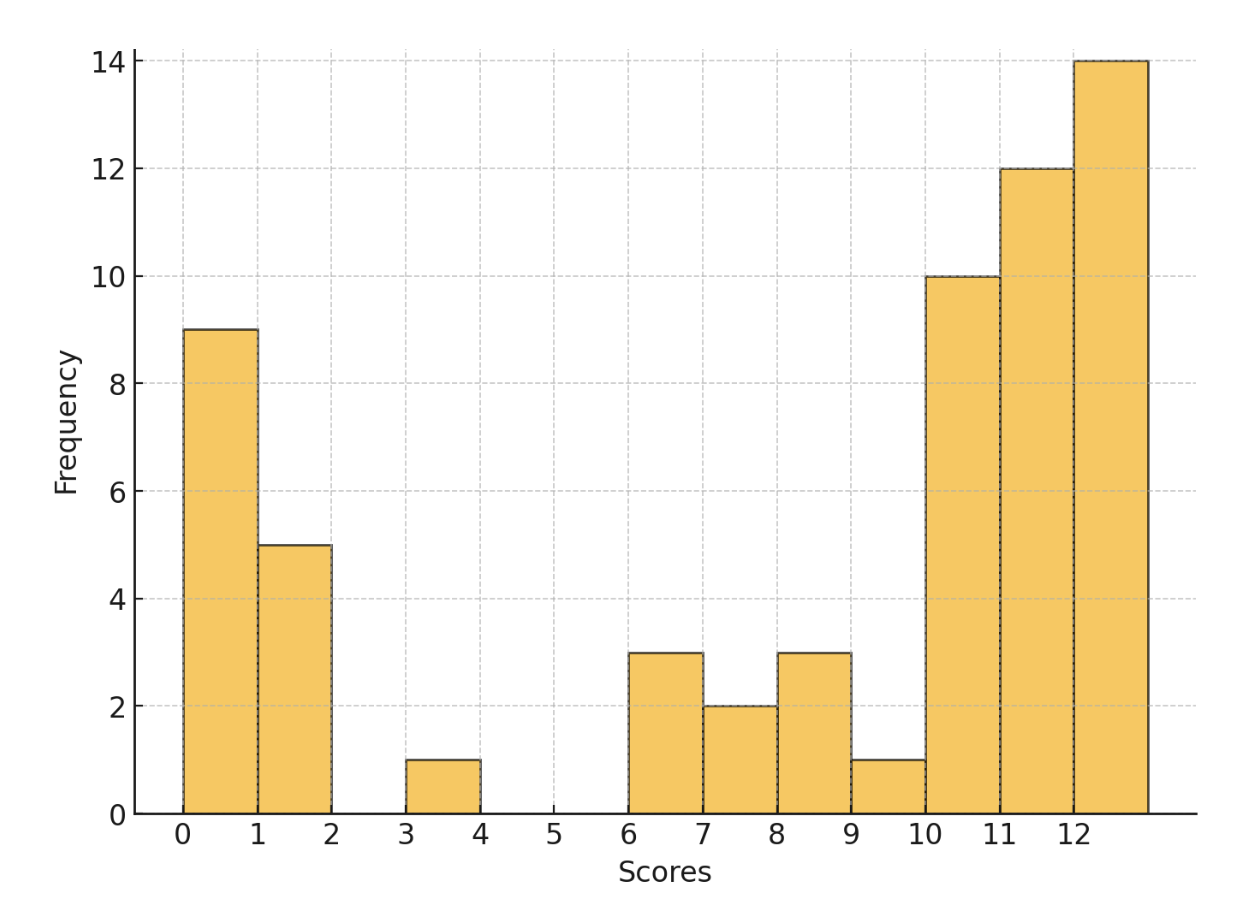
\includegraphics[width=.75\textwidth]{images/reading_quiz_scores}
        \caption{Median Total Score = 10.3/10 (103\%)}
\end{figure}
\vfill 
\textbf{Formula for total score.} A total score was given out of 10. This was obtained by taking 5 times your score on the reading quiz question (2 pts total)  and adding half of your extra credit score (scored out of 4). 
\end{frame}


\begin{frame}{Reading Quiz: Extra Credit Scores}
\footnotesize 
\begin{figure}[ht]
        \centering
        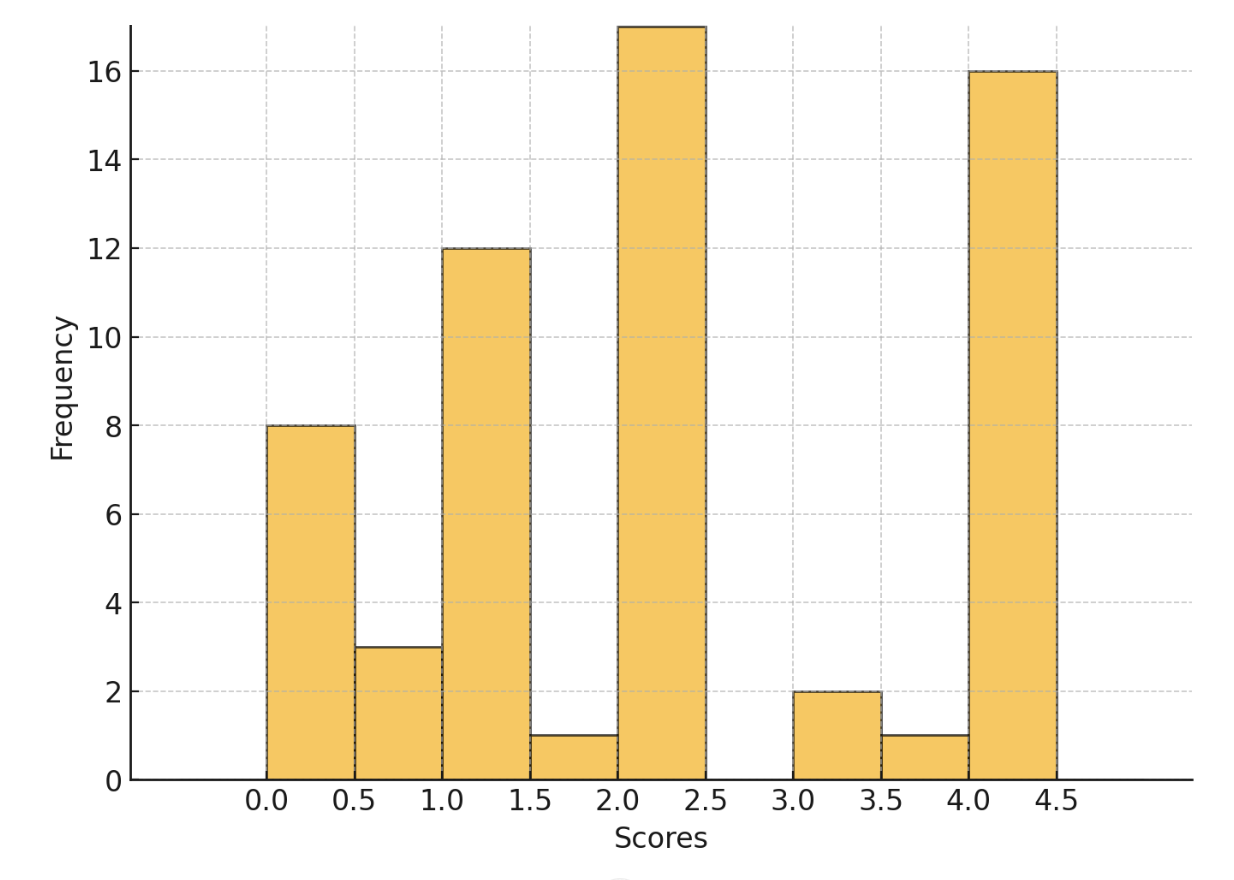
\includegraphics[width=.75\textwidth]{images/ec_quiz_scores}
   		 \caption{Median E.C. Score = 2/4 (50\%)}
\end{figure}
\vfill 
\textbf{Remark.} Most people chose the set equality question. There were various issues with this that we will discuss in class today.  \alertstar Make sure you can answer the set equality question correctly for Friday's problems quiz \alertstar.
\end{frame}


\begin{frame}[standout]
Feedback on Sets I 
\end{frame}




\begin{frame}

 \begin{mygreenbox}[title=Problem]
Prove that the following two sets are equal:
%
\begin{align*}
E &= \set{x \in \mathbb{Z}: x \text{\; is even}}, \text{and} \\
F &= \set{x \in \mathbb{Z}: x=a+b, \text{where $a$ and $b$ are both odd}}
\end{align*}
\end{mygreenbox}

\vfill 
 \begin{myyellowbox}[title=Puzzle]
Evaluate the student solution below. 
\end{myyellowbox}

\vfill 
 \begin{myredbox}[title=Student Solution]
If $a$ and $b$ are both odd, then we can write $a=2c+1$ and $b=2d+1$, where both $c$ and $d$ are integers.  Now 
\[ a+b = (2c+1) + (2d+1) = 2c+2d+2 = 2(c+d+1).\]
That is, $a+b=2e$, where $e \defeq c+d+1$.  Hence, $a+b$ is even.  Hence,  the sets $E$ and $F$ are equal. 
\end{myredbox}
\end{frame}


\begin{frame}{How to show two sets are equal}


 \begin{mygreenbox}[title=Proving two sets are equal]
To show $A=B$, we show $A \subseteq B$ and $B \subseteq A$.
\begin{itemize}
\item $\boxed{A \subseteq B.}$ We show that if $x \in A $, then $x \in B$.  
\item $\boxed{B \subseteq A.}$	We show that if $x \in B$, then $x \in A$.
\end{itemize}
\end{mygreenbox}	
\pause 
\begin{myredbox}[title=Visualization]

\begin{minipage}{0.48\textwidth}
\centering
\footnotesize The first bulletpoint shows
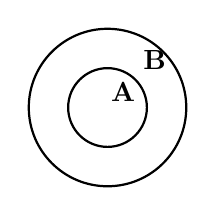
\begin{tikzpicture}
    % Draw Set B (larger set)
    \draw[thick] (0,0) circle (1.0cm);
    \node at (0.6,0.6) {\textbf{B}};

    % Draw Set A (nested inside B)
    \draw[thick] (0,0) circle (0.5cm);
    \node at (0.2,0.2) {\textbf{A}};
\end{tikzpicture}
\end{minipage}
\begin{minipage}{0.48\textwidth}
\centering
\footnotesize  The second bulletpoint shows
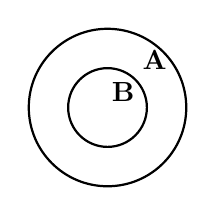
\begin{tikzpicture}
    % Draw Set B (larger set)
    \draw[thick] (0,0) circle (1.0cm);
    \node at (0.6,0.6) {\textbf{A}};

    % Draw Set A (nested inside B)
    \draw[thick] (0,0) circle (0.5cm);
    \node at (0.2,0.2) {\textbf{B}};
\end{tikzpicture}
\end{minipage}
\vfill
\centering 
Therefore
\vspace{0.1cm}
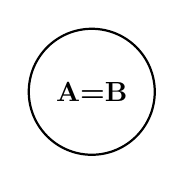
\begin{tikzpicture}
    % Draw Set B (larger set)
    \draw[thick] (0,0) circle (0.8cm);
    \node at (0.0,0.0) {\textbf{A=B}};
\end{tikzpicture}


\end{myredbox}

\end{frame}


\begin{frame}{Solution to problem}


\textbf{Problem.} 
Prove that the following two sets are equal:
%
\begin{align*}
E &= \set{x \in \mathbb{Z}: x \text{\; is even}}, \text{and} \\
F &= \set{x \in \mathbb{Z}: x=a+b, \text{where $a$ and $b$ are both odd}}
\end{align*}


\vfill 
\textbf{Solution.} To show $E=F$, we show $E \subseteq F$ and $F \subseteq E$.
\begin{itemize}
\item $\boxed{E \subseteq F.}$ We show that if $x \in E $, then $x \in F$.  Let $x \in E$.  Then $x=2a$ for some integer $a$.  Now we write	
\[ x=2a = \explaintermbrace{odd (by def.)}{(2a+1)} + \explaintermbrace{odd}{(-1)}\]  Hence $x$ is the sum of two odd numbers.  Hence  $x \in F$.
\item $\boxed{F \subseteq E.}$	We show that if $x \in F$, then $x \in E$. Let $x \in F$.  Hence $x=a+b$ for odd integers $a,b$.  By the definition of odd, we can write $a=(2c+1)$ and $b=(2d+1)$ for integers $c,d$.  Hence
\[x= a+b = (2c+1) + (2d+1) = 2c+2d+2 = 2 (c+d+1) \] 
That is, $a+b=2e$, where $e \defeq c+d+1$.  Hence, $a+b$ is even. Hence, $x \in F$.
\end{itemize}

\end{frame}


\begin{frame}[standout]
Q\&A on the Group Exercises for Sets, Part I 
\end{frame}


\begin{frame}
\footnotesize
Group 1: jack.fry,caitlin.hermanson,luka.derry\\
Group 2: joseph.triem,alexander.goetz,mason.barnocky\\
Group 3: lucas.jones6,evan.schoening,ethan.johnson18\\
Group 4: ryan.barrett2,jonas.zeiler,alexander.knutson\\
Group 5: anthony.mann,kaden.price,jett.girard\\
Group 6: nolan.scott1,devon.maurer,jacob.ruiz1\\
Group 7: jacob.shepherd1,joseph.mergenthaler,zeke.baumann\\
Group 8: peter.buckley1,jacob.ketola,derek.price4\\
Group 9: timothy.true,griffin.short,tyler.broesel\\
Group 10: jakob.kominsky,erik.moore3,yebin.wallace\\
Group 11: adam.wyszynski,connor.yetter,john.fotheringham\\
Group 12: james.brubaker,colter.huber,matthew.nagel\\
Group 13: aaron.loomis,delaney.rubb,conner.reed1\\
Group 14: carver.wambold,lynsey.read,blake.leone\\
Group 15: tristan.nogacki,luke.donaldson1,samuel.mosier\\
Group 16: michael.oswald,justice.mosso,pendleton.johnston\\
Group 17: jada.zorn,emmeri.grooms,micaylyn.parker\\
Group 18: samuel.hemmen,bridger.voss,carsten.brooks\\
Group 19: sarah.periolat,connor.mizner,cameron.wittrock\\
Group 20: evan.barth,reid.pickert,connor.graville\\
Group 21: william.elder1,peyton.trigg,samuel.rollins\\
Group 22: jeremiah.mackey,julia.larsen,owen.obrien\\\end{frame}


\begin{frame}{Group exercises: Quantifiers}

\footnotesize 
\begin{minipage}{0.56\textwidth}
    1. Label each sentence below about the integers as true or false. 
    \begin{itemize}
        \item[a.] $\forall x, \forall y, x+y=0.$ 
        \item[b.] $\forall x, \exists y: x+y=0.$
        \item[c.] $\exists x: \forall y, x+y=0.$
        \item[d.] $\exists x, \exists y: x+y=0.$
        \item[e.] $\forall x, \forall y, xy=0.$
        \item[f.] $\forall x, \exists y: xy=0.$
        \item[g.] $\exists x: \forall y, xy=0.$
        \item[h.] $\exists x, \exists y: xy=0.$
    \end{itemize}
    2. The notation $\exists!$ can be read "there is a unique." Label each sentence below true or false.
    \vspace{-0.5cm}
    \begin{itemize}
        \item[a.] $\exists! x \in \mathbb{N}: x^2=4.$ 
        \item[b.] $\exists! x \in \mathbb{Z}: x^2=4.$ 
        \item[c.] $\exists! x \in \mathbb{N}: x^2=3.$ 
        \item[d.] $\exists! x \in \mathbb{Z}: \forall y \in \mathbb{Z}, xy=x.$ 
        \item[e.] $\exists! x \in \mathbb{Z}: \forall y \in \mathbb{Z}, xy=y.$ 
    \end{itemize}
\end{minipage}
\hfill
\begin{minipage}{0.38\textwidth}
    3. For each sentence below, write the negation of the sentence, but place the $\lnot$ symbol as far to the right as possible. Then rewrite the negation in English.  The first problem is done for you.
    \begin{itemize}
    
        \item[a.] $\forall x \in \mathbb{Z}, x \text{ is odd.} $  \alert{Solution: $\exists x \in \mathbb{Z}: \lnot (x \text{ is odd}.)$. In English: "There is an integer which is not odd."}
        \item[b.] $\forall x \in \mathbb{Z}, x<0.$ 
        \item[c.] $\exists x \in \mathbb{Z}: x=x+1.$
        \item[d.] $\exists x \in \mathbb{N}: x>10.$
        \item[e.] $\forall x \in \mathbb{N}, x+x=2x.$
        \item[f.] $\exists x \in \mathbb{Z}: \forall y \in \mathbb{Z}, x>y.$
        \item[g.]  $\forall x \in \mathbb{Z}, \forall y \in \mathbb{Z}, x=y.$
        \item[h.] $\forall x \in \mathbb{Z}, \exists y \in \mathbb{Z}: x+y=0.$
    \end{itemize}
\end{minipage}

\end{frame}



\end{document}
